\section{Оптимизация геометрических параметров сечения центроплана}
\subsection{Постановка задачи}
В ходе работы было проведено исследование зависимости веса центроплана от его параметров с учетом критерия неразрушения конструкции при заданных нагрузках. Для этого была решена следующая модельная задача.

\subsection{Постановка модельной задачи}
Имеется упрощенная модель центроплана -- короб переменного прямоугольного сечения с перегородками. На него передаются нагрузки посредством приложения аэродинамических нагрузок на модель крыла -- короб постоянного прямоугольного сечения. Для модели центроплана имеются два параметра: относительная координата нижней точки сечения и строительная высота в плоскости симметрии самолета. Было выбрано 42 пары параметров, для каждой пары проведена оптимизация сечения с целью удовлетворения требований прочности конструкции, а именно: среднее напряжение в каждой панели не должно превышать допускаемого напряжения, равного $35\text{кг}/\text{мм}^2$. Оптимизация проводилась алгоритмом $\sigma/\sigma$ для каждой панели. Итоговые результаты вычислений приведены в таблице \ref{tab:KessOptimBigTable} и на Рис.\ref{fig:Optimization3dplot}

\tabulinesep = 1mm
\definecolor{lightgray}{gray}{0.9}
\begin{table}[H]
\captionsetup{justification=centering}
\caption{Зависимость площади панелей центроплана и веса кессона от параметров центроплана}
%\rowcolors{2}{}{lightgray}
\begin{tabu}to \linewidth{|c|*4{X[m c]|}*4{X[m c]|}}
\hline
\multirow{2}{*}[-1.1ex]{N} & \multicolumn{4}{c|}{Вес кессона~[кг]} & \multicolumn{4}{c|}{Площадь панелей центроплана~[$\text{м}^2$]} \\ \cline{2-9}
& Верхние панели & Нижние панели & Боковые стенки & $\Sigma$ & Верхние панели & Нижние панели & Боковые стенки & $\Sigma$ \\
\hline
\taburowcolors {lightgray .. white}
1 & 297.182 & 294.551 & 12.561 & 604.294 & 2.730 & 2.730 & 4.000 & 9.520\\ \hline
2 & 225.261 & 237.378 & 27.672 & 490.313 & 2.730 & 2.740 & 5.210 & 10.720\\ \hline
3 & 190.080 & 222.327 & 49.159 & 461.564 & 2.730 & 2.760 & 5.820 & 11.340\\ \hline
4 & 161.544 & 211.467 & 65.963 & 438.972 & 2.730 & 2.760 & 6.450 & 11.950\\ \hline
5 & 146.581 & 199.989 & 66.844 & 413.415 & 2.730 & 2.780 & 7.090 & 12.590\\ \hline
6 & 134.746 & 191.293 & 70.912 & 396.952 & 2.730 & 2.800 & 7.640 & 13.200\\ \hline
7 & 350.816 & 374.021 & 47.679 & 772.515 & 2.910 & 2.910 & 4.000 & 9.850\\ \hline
8 & 253.752 & 259.311 & 53.180 & 566.245 & 2.910 & 2.850 & 5.210 & 10.990\\ \hline
9 & 213.881 & 226.655 & 57.618 & 498.154 & 2.910 & 2.830 & 5.840 & 11.570\\ \hline
10 & 188.442 & 205.603 & 62.047 & 456.092 & 2.910 & 2.810 & 6.450 & 12.150\\ \hline
11 & 174.466 & 196.192 & 66.506 & 437.164 & 2.910 & 2.780 & 7.090 & 12.770\\ \hline
12 & 154.328 & 195.919 & 70.963 & 421.210 & 2.910 & 2.770 & 7.680 & 13.350\\ \hline
13 & 363.681 & 391.414 & 48.862 & 803.953 & 3.010 & 3.000 & 4.000 & 10.000\\ \hline
14 & 258.118 & 275.555 & 53.209 & 586.883 & 3.010 & 2.930 & 5.230 & 11.160\\ \hline
15 & 225.322 & 238.220 & 57.604 & 521.145 & 3.010 & 2.890 & 5.820 & 11.720\\ \hline
16 & 201.612 & 214.755 & 62.046 & 478.413 & 3.010 & 2.860 & 6.440 & 12.310\\ \hline
17 & 171.877 & 203.370 & 66.418 & 441.665 & 3.010 & 2.840 & 7.050 & 12.900\\ \hline
18 & 163.553 & 201.207 & 70.912 & 435.673 & 3.010 & 2.820 & 7.660 & 13.480\\ \hline
19 & 380.079 & 398.521 & 49.032 & 827.631 & 3.050 & 3.050 & 4.000 & 10.110\\ \hline
20 & 267.143 & 279.590 & 53.134 & 599.866 & 3.050 & 2.980 & 5.210 & 11.240\\ \hline
21 & 231.158 & 238.954 & 57.667 & 527.779 & 3.050 & 2.930 & 5.820 & 11.820\\ \hline
22 & 197.327 & 218.001 & 62.040 & 477.368 & 3.050 & 2.910 & 6.410 & 12.390\\ \hline
23 & 191.553 & 205.935 & 66.481 & 463.971 & 3.050 & 2.870 & 7.070 & 12.980\\ \hline
24 & 158.352 & 203.948 & 70.897 & 433.199 & 3.050 & 2.850 & 7.660 & 13.560\\ \hline
25 & 383.525 & 410.374 & 50.351 & 844.249 & 3.110 & 3.110 & 4.000 & 10.210\\ \hline
26 & 279.228 & 288.331 & 53.186 & 620.745 & 3.110 & 3.030 & 5.210 & 11.350\\ \hline
27 & 233.614 & 249.500 & 57.583 & 540.696 & 3.110 & 2.990 & 5.820 & 11.910\\ \hline
28 & 213.922 & 221.683 & 62.125 & 497.728 & 3.110 & 2.950 & 6.450 & 12.500\\ \hline
29 & 180.457 & 210.067 & 66.523 & 457.046 & 3.110 & 2.920 & 7.070 & 13.070\\ \hline
30 & 167.492 & 205.426 & 71.001 & 443.918 & 3.110 & 2.880 & 7.640 & 13.660\\ \hline
31 & 401.418 & 424.040 & 50.413 & 875.868 & 3.160 & 3.160 & 4.000 & 10.330\\ \hline
32 & 285.115 & 297.451 & 53.649 & 636.214 & 3.160 & 3.070 & 5.230 & 11.470\\ \hline
33 & 251.131 & 255.015 & 57.656 & 563.801 & 3.160 & 3.040 & 5.860 & 12.030\\ \hline
34 & 212.049 & 229.543 & 62.067 & 503.658 & 3.160 & 3.000 & 6.450 & 12.610\\ \hline
35 & 191.030 & 215.968 & 66.550 & 473.548 & 3.160 & 2.970 & 7.070 & 13.170\\ \hline
36 & 170.765 & 209.184 & 70.962 & 450.912 & 3.160 & 2.920 & 7.660 & 13.740\\ \hline
37 & 431.880 & 451.562 & 51.974 & 935.418 & 3.230 & 3.230 & 4.000 & 10.440\\ \hline
38 & 291.199 & 306.178 & 54.263 & 651.640 & 3.230 & 3.130 & 5.210 & 11.560\\ \hline
39 & 253.054 & 265.073 & 57.593 & 575.719 & 3.230 & 3.090 & 5.820 & 12.140\\ \hline
40 & 222.782 & 233.403 & 61.948 & 518.132 & 3.230 & 3.050 & 6.400 & 12.700\\ \hline
41 & 197.192 & 218.301 & 66.423 & 481.917 & 3.230 & 3.020 & 7.030 & 13.270\\ \hline
42 & 175.591 & 210.828 & 70.877 & 457.295 & 3.230 & 2.970 & 7.660 & 13.840\\ \hline
\end{tabu}

\label{tab:KessOptimBigTable}
\end{table}

\begin{landscape}
\begin{figure}[ht]
\captionsetup{justification=centering}
\caption{Зависимость веса кессона от параметров центроплана}
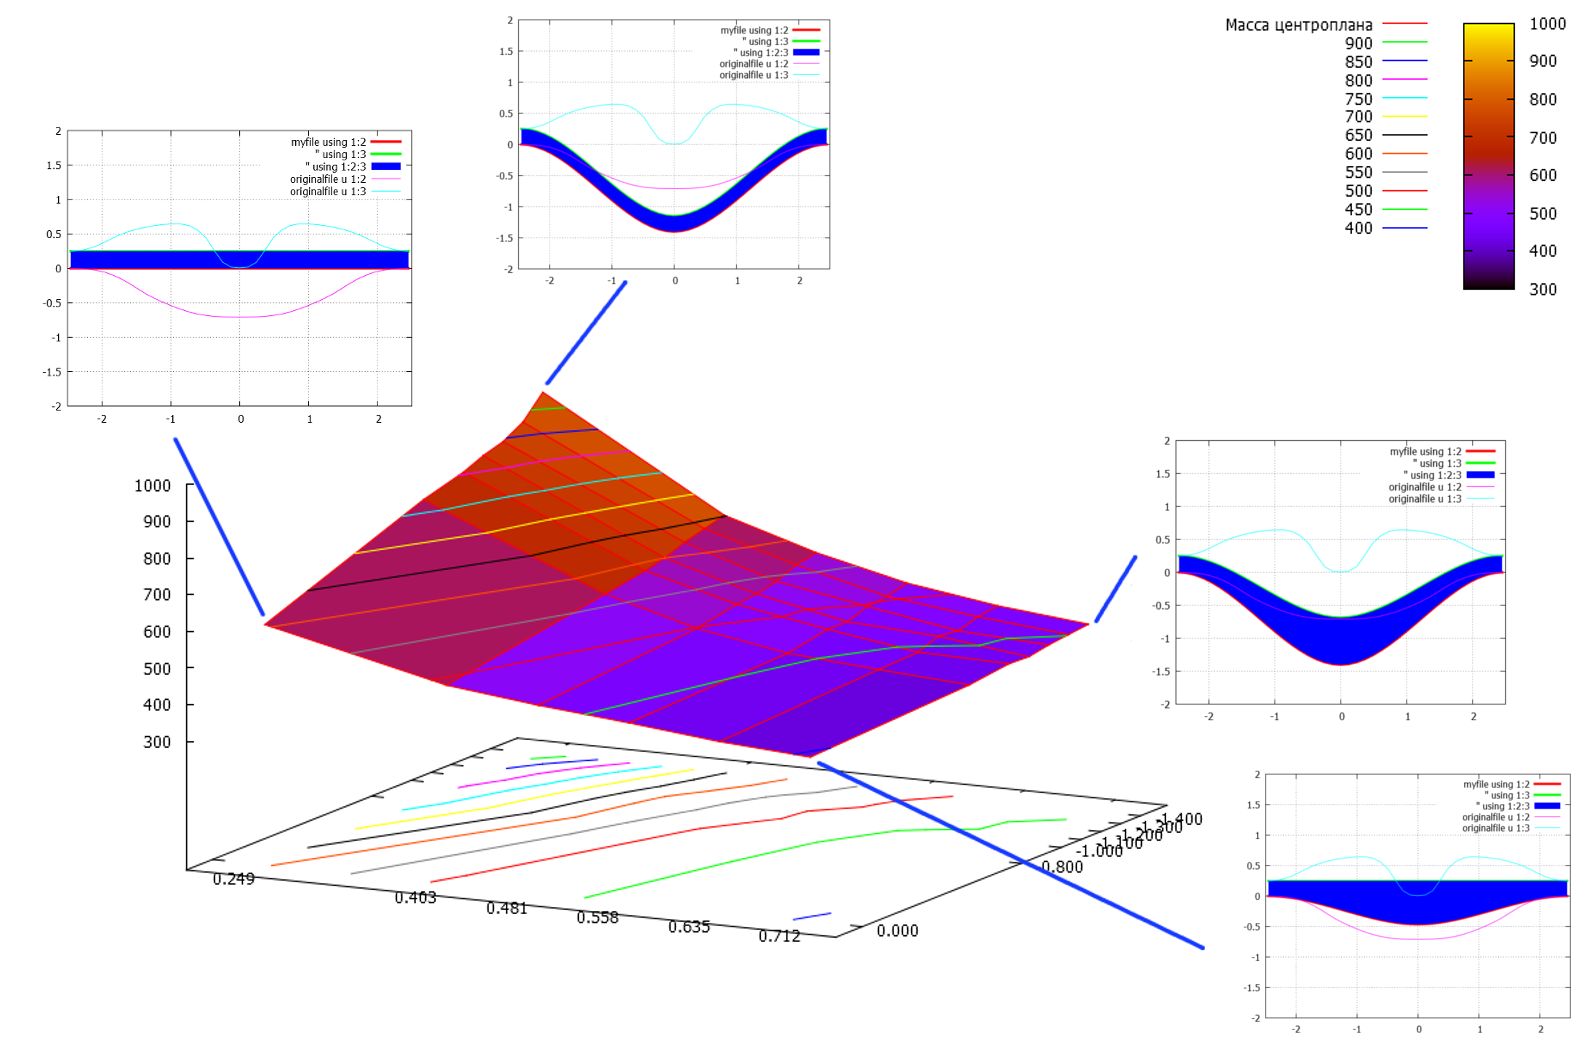
\includegraphics[height=0.9\textwidth]{Optimization3dplot}
\label{fig:Optimization3dplot}
\end{figure}
\end{landscape}


